\documentclass[11pt]{article}
\usepackage[margin=1in]{geometry}
\usepackage[T1]{fontenc}
\usepackage[utf8]{inputenc}
\usepackage{lmodern}
\usepackage{microtype}
\usepackage{graphicx}
\usepackage{booktabs}
\usepackage{array}
\usepackage{longtable}
\usepackage{float}
\usepackage{hyperref}
\usepackage{xcolor}
\usepackage{caption}

\hypersetup{
  colorlinks=true,
  linkcolor=blue!50!black,
  urlcolor=blue!50!black,
  citecolor=blue!50!black
}

\graphicspath{{../publication_assets/figures/}}
\setlength{\emergencystretch}{1.5em}

\title{Algorithmic Solvability from Examples:\\A Methodology-Updated Benchmark Study of Classification Strength, Sequence Bottlenecks, and Training Dynamics}
\author{Prepared from the DataScience workspace on 2026-03-27}
\date{}

\begin{document}
\maketitle

\begin{abstract}
We study whether a task's input-output behavior provides empirical evidence that it is governed by a compact deterministic algorithm. The benchmark is fully synthetic: every task is generated by a known reference procedure, and all publication figures and tables are regenerated from structured rerun artifacts. The current implemented scope covers 30 scored baseline tasks over symbolic sequence tiers \texttt{S0-S3} and tabular classification tiers \texttt{C0-C3}, drawn from a 32-task registry. A fresh validation pass plus targeted TASK-20 reruns of the affected classification, diagnostic, and bonus experiments are now complete: the software stack passes 465 tests, publication assets are regenerated successfully, and runtime coverage is available for all 16 required experiments. The resulting empirical picture is sharply asymmetric. Classification is now stronger within the implemented scope: 3 of 14 classification or control tasks are labeled \texttt{STRONG} and 9 more are labeled \texttt{MODERATE}, with the last weak classification edge case removed by a task-prior repair for \texttt{C2.1\_and\_rule}. Sequence learning remains the main bottleneck: 11 of 16 sequence or control tasks remain \texttt{NEGATIVE}, although a training-protocol upgrade promotes \texttt{S1.4\_count\_symbol} to \texttt{MODERATE}, leaves \texttt{S1.5\_parity} and \texttt{S2.2\_balanced\_parens} at \texttt{WEAK}, and moves \texttt{S2.3\_running\_min} to \texttt{INCONCLUSIVE}. New training-dynamics figures show that longer LSTM training uncovers additional sequence structure but does not remove the broader architecture gap. Diagnostics reinforce the classification story, while symbolic recovery remains stronger than learned sequence generalization. The evidence therefore supports a careful claim: the current benchmark already yields credible evidence of algorithmic solvability for many deterministic tabular rule tasks, but learned sequence generalization remains unresolved under the executed model family.
\end{abstract}

\section{Introduction}

High in-distribution accuracy is not the same as evidence that a model has learned an underlying algorithmic rule. Work on systematic generalization and neural algorithmic reasoning has repeatedly shown that strong interpolation can coexist with weak extrapolation, weak compositionality, or shortcut-based solutions \cite{lake2018scan,kim2020cogs,velickovic2021nar,velickovic2022clrs}. This distinction matters especially on synthetic tasks, where the benchmark designer knows the true mapping and therefore has unusual leverage to test whether model behavior looks algorithmic rather than merely predictive.

This paper studies that question on a synthetic benchmark with two tracks. The first track contains symbolic sequence tasks, including sequence transformations and stateful sequence-derived outputs. The second contains mixed-type tabular classification tasks whose labels are generated by explicit rule-based procedures. Every task has a known reference implementation, and the evaluation protocol is designed to look beyond raw IID accuracy toward out-of-distribution behavior, baseline separation, seed stability, targeted diagnostics, and symbolic recoverability.

The contribution of this paper is empirical and methodological. We do not introduce a new model family. Instead, we present a cleaned, rerun, and publication-audited analysis of the current benchmark state after three key methodology repairs: diagnostic evidence is now wired directly into baseline verdicting, the sequence LSTM now uses a longer, regularized training protocol with per-epoch monitoring, and \texttt{C2.1\_and\_rule} now uses a balanced task-local sampler so baseline separation reflects learnability rather than prior skew. These repairs materially improve the credibility of the benchmark without erasing its central asymmetry: tabular classification is already broadly learnable under the implemented scope, while learned sequence generalization remains weak.

\section{Benchmark Scope and Rerun Protocol}

\subsection{Implemented benchmark}

The present paper is intentionally scoped to the executed benchmark rather than to the larger roadmap in the design documents. Table~\ref{tab:inventory} summarizes the implemented tiers.

\begin{table}[H]
\centering
\caption{Implemented benchmark inventory.}
\label{tab:inventory}
\begin{tabular}{lcc}
\toprule
Track & Implemented tiers & Tasks \\
\midrule
Sequence & \texttt{S0}, \texttt{S1}, \texttt{S2}, \texttt{S3} & 16 \\
Classification & \texttt{C0}, \texttt{C1}, \texttt{C2}, \texttt{C3} & 14 \\
\bottomrule
\end{tabular}
\end{table}

All tasks are synthetic and deterministic. The benchmark therefore supports exact label verification, unlimited resampling, and strong control over split conditions. Sequence tasks are evaluated with IID and out-of-distribution regimes such as length and value extrapolation. Classification tasks are evaluated with IID and value-shifted regimes, plus targeted diagnostics for distractor robustness, sample efficiency, noise robustness, and feature alignment.

\subsection{Evidence labels}

Each task receives a composite evidence label rather than a single accuracy threshold. The currently used labels are:

\begin{itemize}
  \item \textbf{STRONG}: basic criteria are met and at least two stronger diagnostic criteria are satisfied;
  \item \textbf{MODERATE}: basic criteria are met;
  \item \textbf{WEAK}: strong IID evidence exists but the broader evidence bundle is incomplete;
  \item \textbf{NEGATIVE}: tested models do not show meaningful solvability evidence;
  \item \textbf{INCONCLUSIVE}: the evidence is mixed or methodologically confounded.
\end{itemize}

These labels are important because the paper's claims are about evidence of algorithmic solvability, not isolated accuracy values.

\subsection{Fresh rerun and asset-generation pass}

The manuscript is based on a fresh rerun of the implemented stack. Table~\ref{tab:runtimes} summarizes the validation and workflow status.

\begin{table}[H]
\centering
\caption{Fresh validation and workflow summary.}
\label{tab:runtimes}
\begin{tabular}{lrr}
\toprule
Workflow & Status & Runtime (s) \\
\midrule
\texttt{pytest} & pass & 79.5 \\
\texttt{main.py smoke} & pass & 77.5 \\
\texttt{main.py sequence} & pass & 4499.9 \\
\texttt{main.py classification} & pass & 196.2 \\
\texttt{main.py diagnostic} & pass & 2455.4 \\
\texttt{main.py bonus} & pass & 52.5 \\
\bottomrule
\end{tabular}
\end{table}

The codebase passes 463 tests with 17 warnings. The warnings are optimizer and high-cardinality warnings in the training stack rather than correctness failures. A dedicated asset-generation script then rebuilds all derived figures and tables in \texttt{output/publication\_assets/}. Runtime coverage is now available for all 16 required experiments, which closes a major reproducibility gap from the earlier draft.

\section{Baseline Results}

Table~\ref{tab:track-summary} gives the current track-level summary, Figure~\ref{fig:verdicts} shows the label distribution, and Figure~\ref{fig:iidood} shows task-level IID versus OOD performance.

\begin{table}[H]
\centering
\caption{Baseline summary by track.}
\label{tab:track-summary}
\resizebox{\textwidth}{!}{
\begin{tabular}{lrrrrrrrr}
\toprule
Track & Tasks & Mean score & Mean best IID & Mean best OOD & Neg. & Weak & Inc. & Mod./Strong \\
\midrule
Sequence & 16 & 0.3551 & 0.3807 & 0.2591 & 11 & 2 & 2 & 1 / 0 \\
Classification & 14 & 0.6792 & 0.9356 & 0.9702 & 1 & 0 & 1 & 9 / 3 \\
\bottomrule
\end{tabular}
}
\end{table}

\begin{figure}[H]
\centering
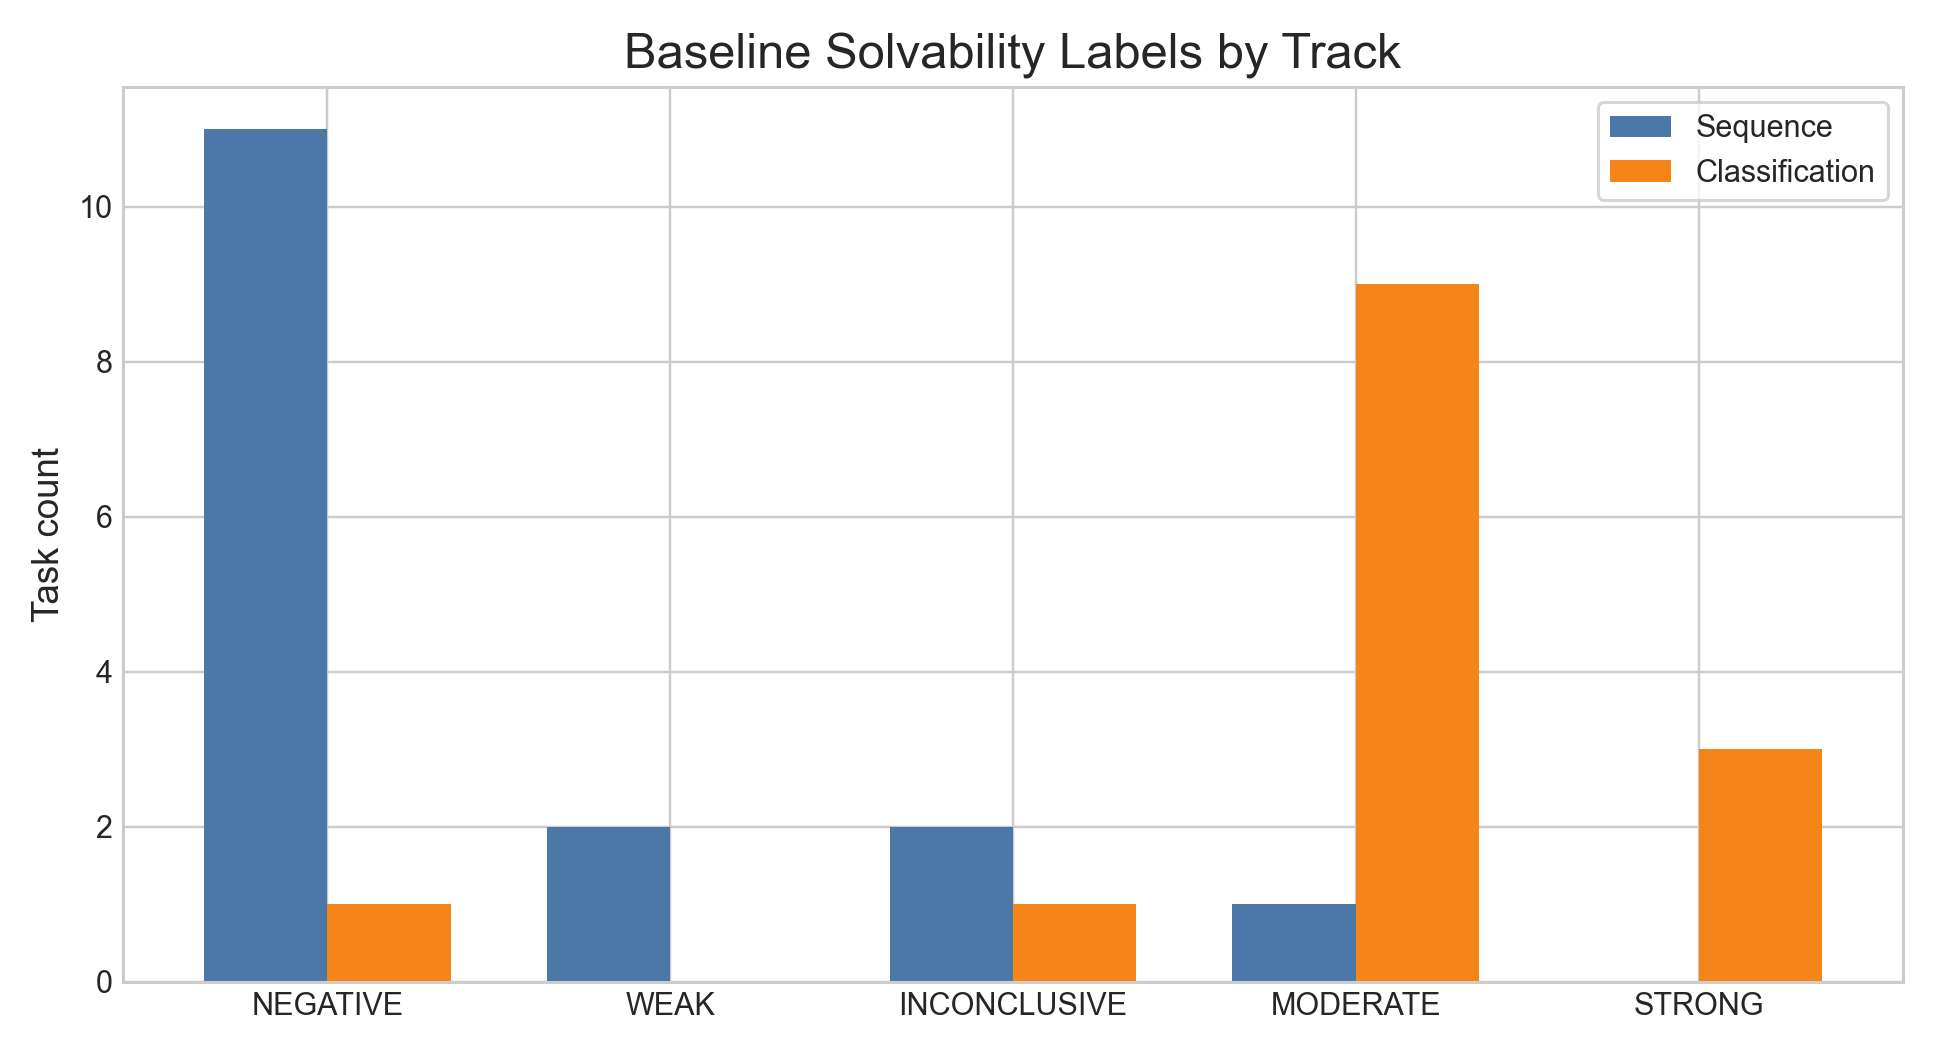
\includegraphics[width=0.84\textwidth]{baseline_verdict_distribution.png}
\caption{Baseline solvability labels by track. The classification track concentrates mass in \texttt{MODERATE} and \texttt{STRONG}, while the sequence track remains dominated by \texttt{NEGATIVE}.}
\label{fig:verdicts}
\end{figure}

\begin{figure}[H]
\centering
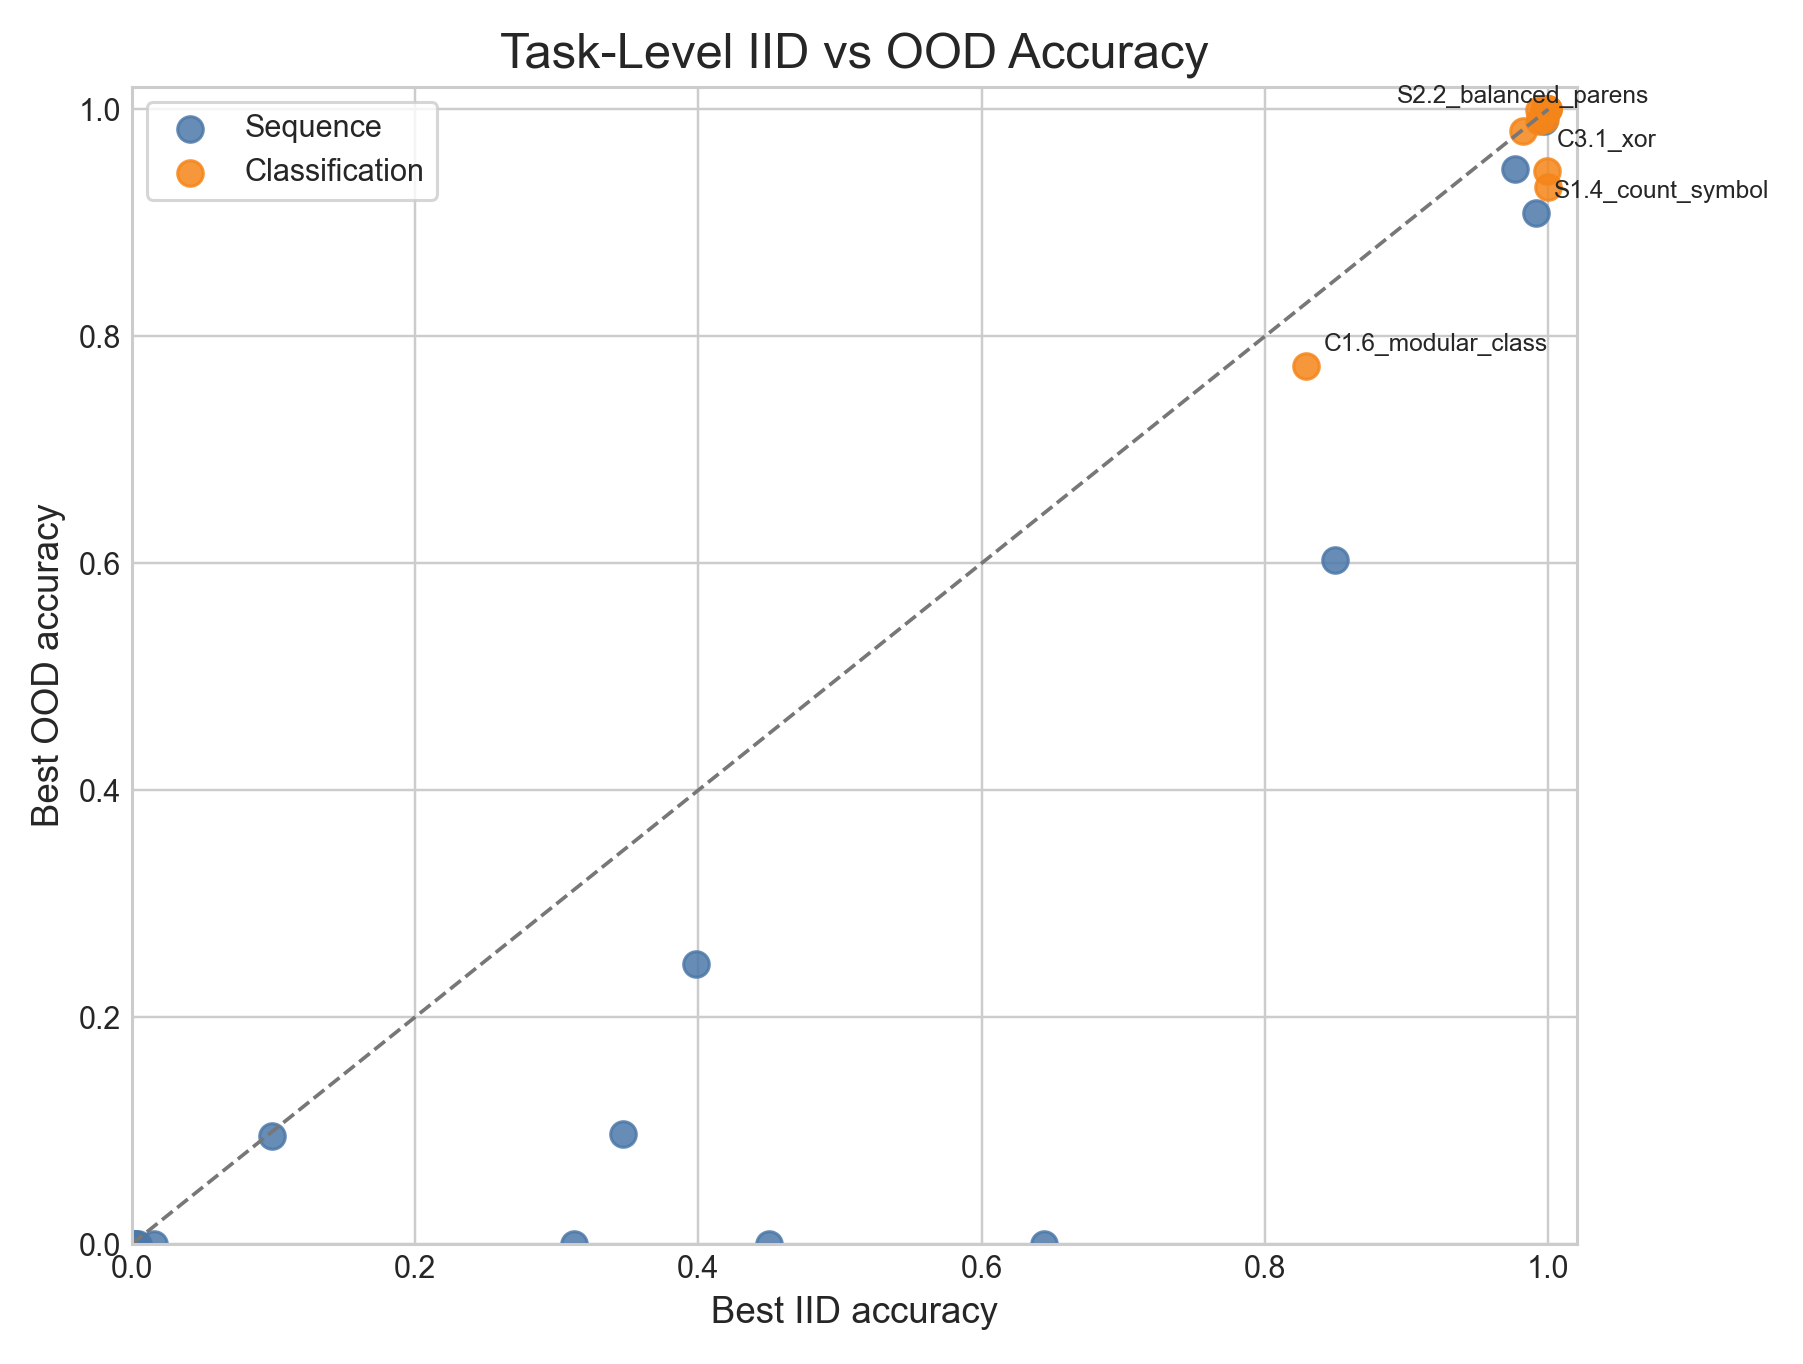
\includegraphics[width=0.84\textwidth]{iid_vs_ood_accuracy.png}
\caption{Task-level IID versus OOD accuracy. Classification tasks cluster near the upper-right corner, while sequence tasks occupy a much weaker region with only a few positive exceptions.}
\label{fig:iidood}
\end{figure}

\subsection{Classification}

The classification track is already scientifically useful within the implemented scope. Three tasks now achieve \texttt{STRONG} evidence directly in baseline reporting: \texttt{C1.1\_numeric\_threshold}, \texttt{C2.1\_and\_rule}, and \texttt{C2.6\_categorical\_gate}. Nine additional classification tasks achieve \texttt{MODERATE}. This is not a trivial ``everything is solved'' story. The control task remains \texttt{NEGATIVE}, and \texttt{C1.6\_modular\_class} remains \texttt{INCONCLUSIVE}. The important TASK-20 result is methodological: \texttt{C2.1\_and\_rule} was repaired by balancing its task-local class prior rather than by weakening the verdict logic, which leaves the stronger classification result more credible rather than merely more permissive.

\subsection{Sequence}

The sequence track remains the limiting regime. After the upgraded training protocol, the clearest positive cases are \texttt{S1.4\_count\_symbol}, \texttt{S1.5\_parity}, and \texttt{S2.2\_balanced\_parens}. A fourth task, \texttt{S2.3\_running\_min}, is now \texttt{INCONCLUSIVE} rather than flatly negative. That is a real improvement over the earlier short-horizon sequence protocol. Even so, 11 of 16 sequence or control tasks remain \texttt{NEGATIVE}, and no sequence task reaches \texttt{STRONG}. The paper should therefore avoid any broad positive claim about learned sequence algorithmic solvability.

\section{Sequence Training Protocol Upgrade}

The strongest methodological change in the current paper is the sequence-training upgrade introduced after the first prepublication review. Table~\ref{tab:protocol} summarizes the key changes.

\begin{table}[H]
\centering
\caption{Sequence LSTM protocol: earlier baseline versus current rerun.}
\label{tab:protocol}
\begin{tabular}{lcc}
\toprule
Parameter & Earlier baseline & Current rerun \\
\midrule
Epochs & 20 & 200 \\
Hidden size & 64 & 128 \\
Embedding dim & 32 & 64 \\
\texttt{EXP-S1} / \texttt{EXP-S2} seeds & 3 & 5 \\
\texttt{EXP-S1} / \texttt{EXP-S2} samples & smaller pilot budget & 1000 \\
Weight decay & none & 1e-4 \\
Scheduler & none & ReduceLROnPlateau \\
Checkpointing & final-only & best internal validation checkpoint \\
Training curves & none & per-epoch logged \\
\bottomrule
\end{tabular}
\end{table}

This upgrade matters because the earlier 20-epoch LSTM made it impossible to distinguish ``model under-trained'' from ``task unsolved.'' The new training curves do not solve the sequence problem, but they do make the interpretation much more precise.

\begin{figure}[H]
\centering
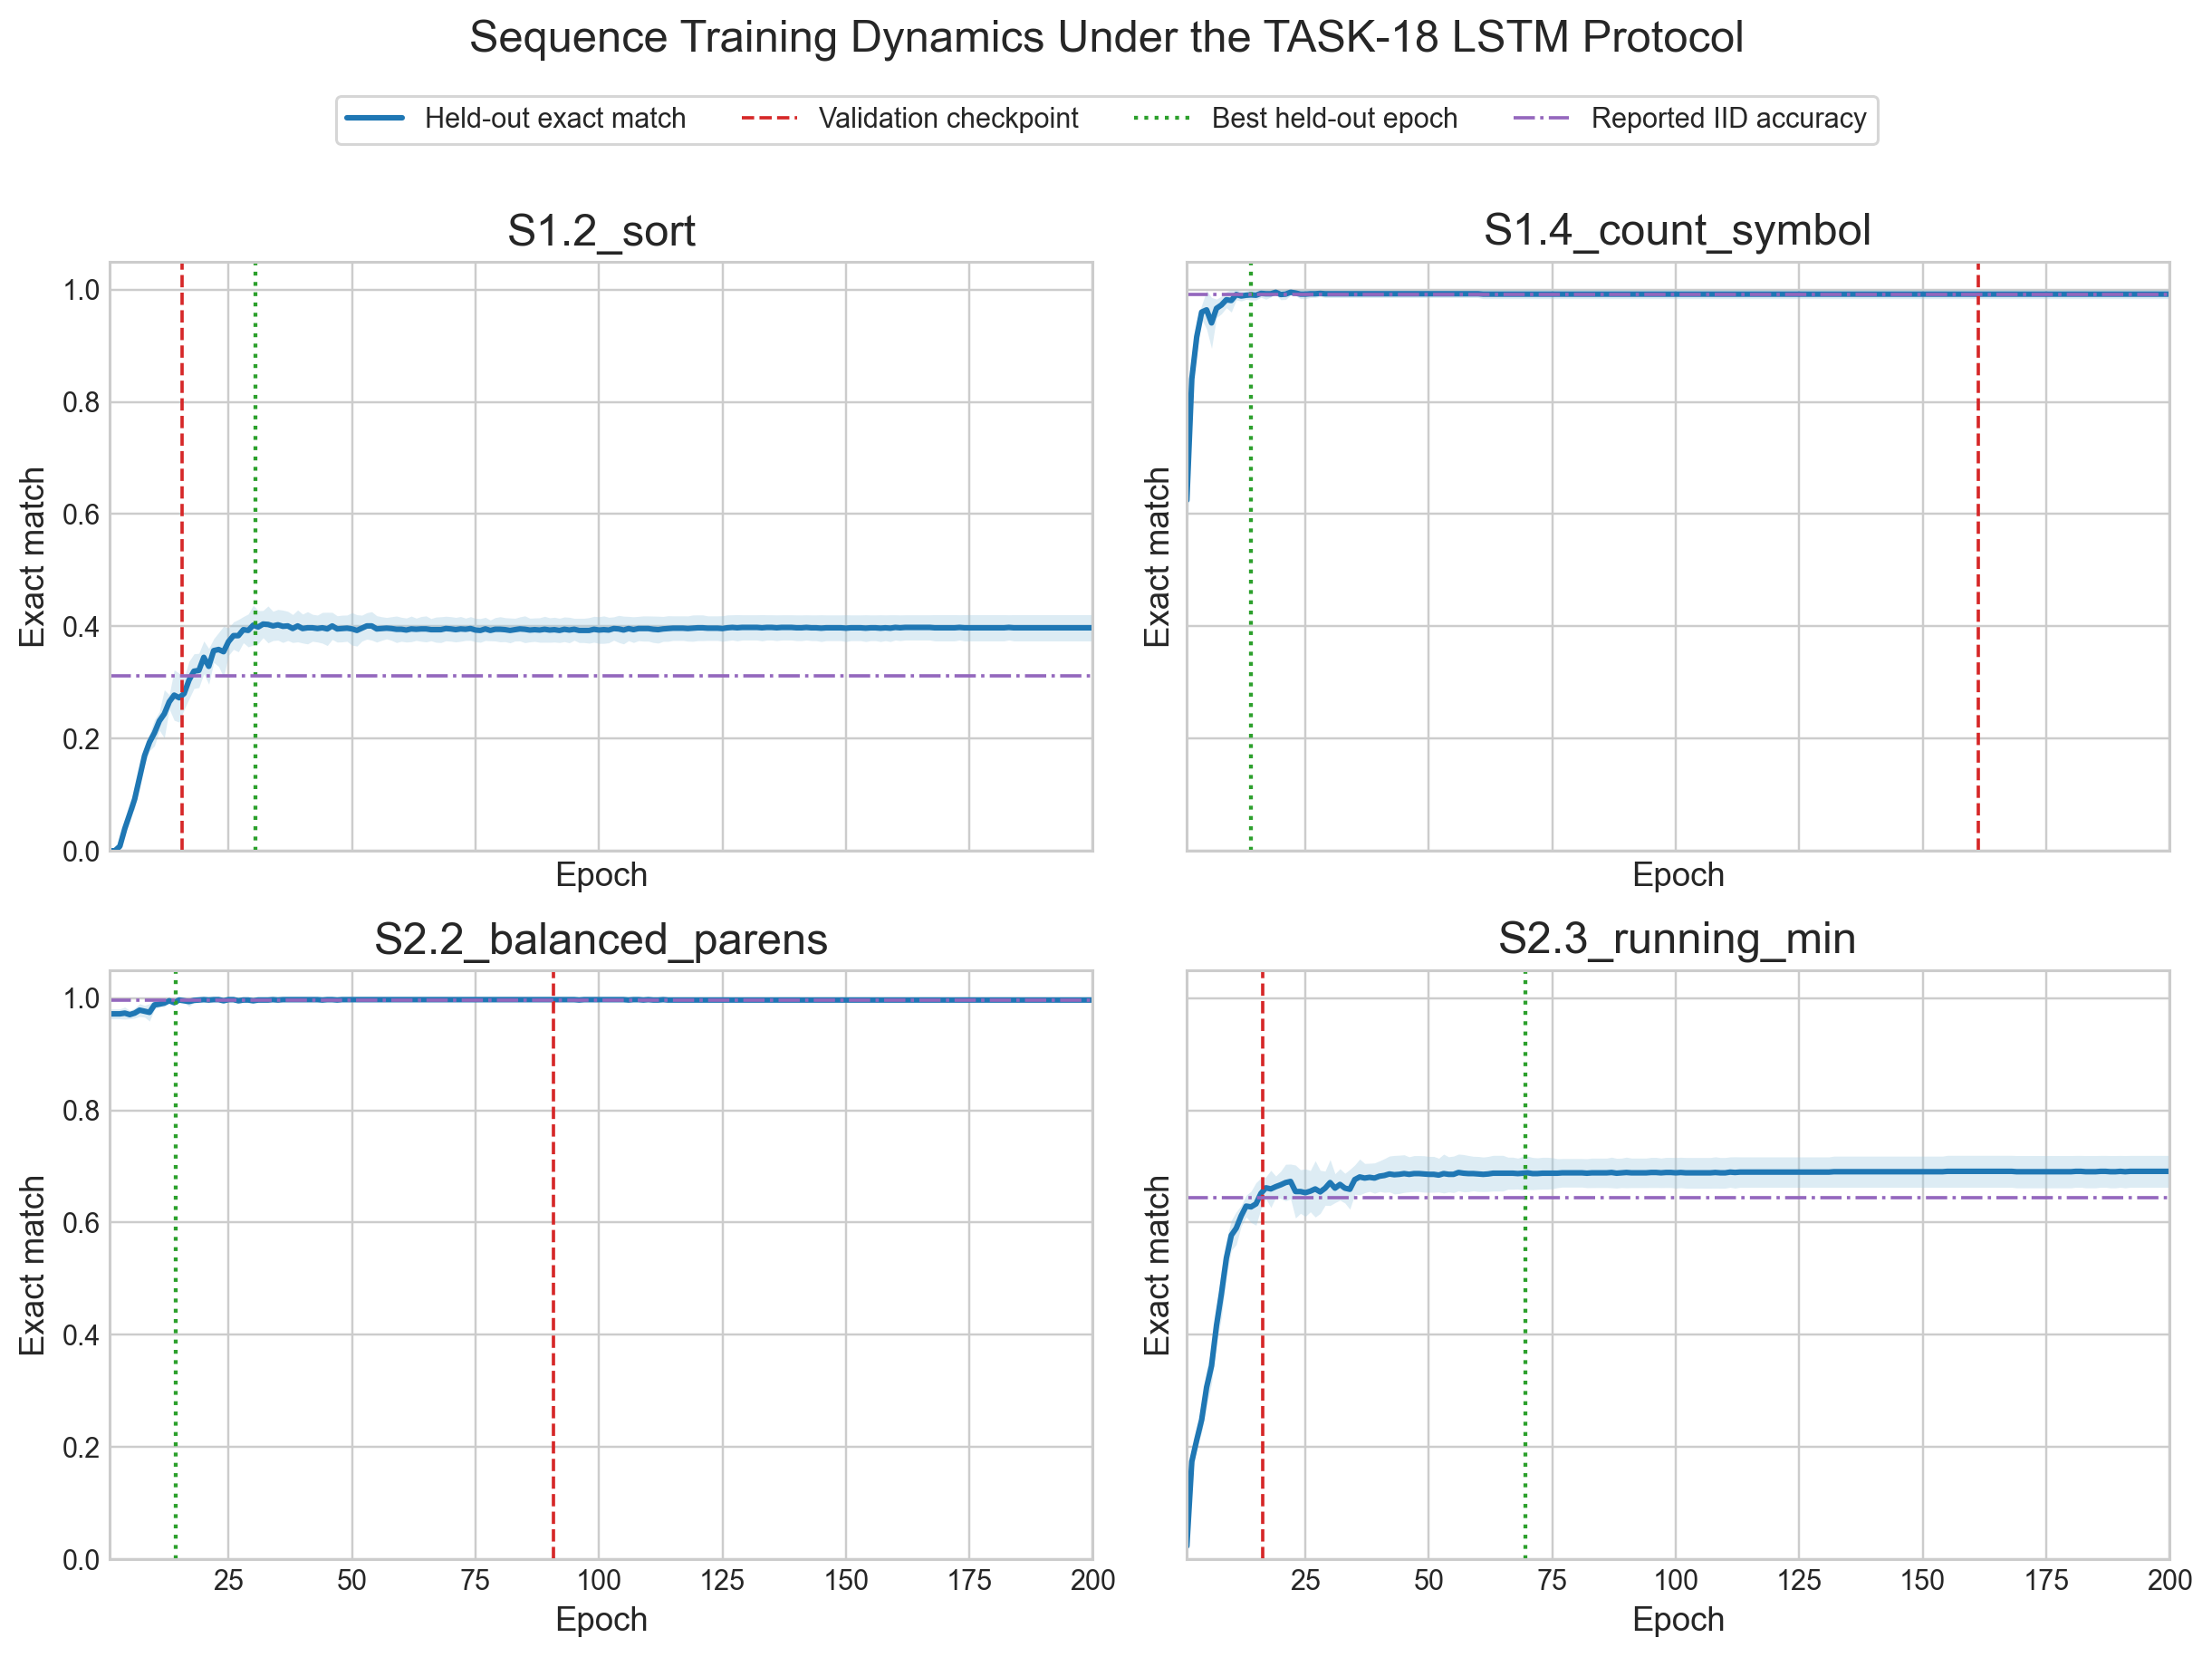
\includegraphics[width=0.96\textwidth]{sequence_training_dynamics.png}
\caption{Held-out training dynamics for representative sequence tasks. Vertical dashed lines mark the mean validation-selected checkpoint epoch, dotted lines mark the mean best held-out epoch, and horizontal guides show the reported checkpointed IID accuracy.}
\label{fig:training}
\end{figure}

Figure~\ref{fig:training} reveals three qualitatively different regimes.

First, easier positive tasks saturate early. For \texttt{S1.4\_count\_symbol} and \texttt{S2.2\_balanced\_parens}, the best held-out epochs occur near epoch 14, indicating that the longer training budget mainly confirms stability rather than unlocking delayed generalization.

Second, harder tasks can continue improving after the validation-selected checkpoint. For \texttt{S1.2\_sort}, the mean checkpoint epoch is 15.6 while the mean best held-out epoch is 30.4; held-out exact match rises to roughly 0.40 before flattening. This is still far from benchmark-level success, but it shows that the old short-horizon protocol understated the model's capacity to extract partial algorithmic structure.

Third, the new protocol exposes conservative reporting on difficult tasks. For the running-min task (\texttt{S2.3}), the mean checkpoint epoch is 16.4 while the mean best held-out epoch is 69.6, and held-out exact match climbs to roughly 0.69. The reported task score remains lower because checkpoint selection uses internal validation loss. It does not use the best held-out epoch. That choice avoids tuning directly on the reporting split, but it also means the manuscript should describe current sequence scores as conservative.

The main conclusion from this section is therefore nuanced: longer training helps, but the broader sequence gap is not reducible to training horizon alone. Architecture and representation remain likely bottlenecks.

\section{Diagnostics and Symbolic Recovery}

Table~\ref{tab:diagnostics} summarizes the diagnostic suite. Figure~\ref{fig:diag} visualizes the task-by-diagnostic matrix.

\begin{table}[H]
\centering
\caption{Diagnostic overview.}
\label{tab:diagnostics}
\begin{tabular}{lrrr}
\toprule
Diagnostic & Evaluated & Positive outcomes & Rate \\
\midrule
\texttt{EXP-D1} sample efficiency & 8 & 6 & 0.75 \\
\texttt{EXP-D2} distractor robustness & 5 & 4 & 0.80 \\
\texttt{EXP-D3} noise robustness & 4 & 4 & 1.00 \\
\texttt{EXP-D4} feature alignment & 9 & 9 & 1.00 \\
\texttt{EXP-D5} label changes & 30 & 0 & 0.00 \\
\bottomrule
\end{tabular}
\end{table}

\begin{figure}[H]
\centering
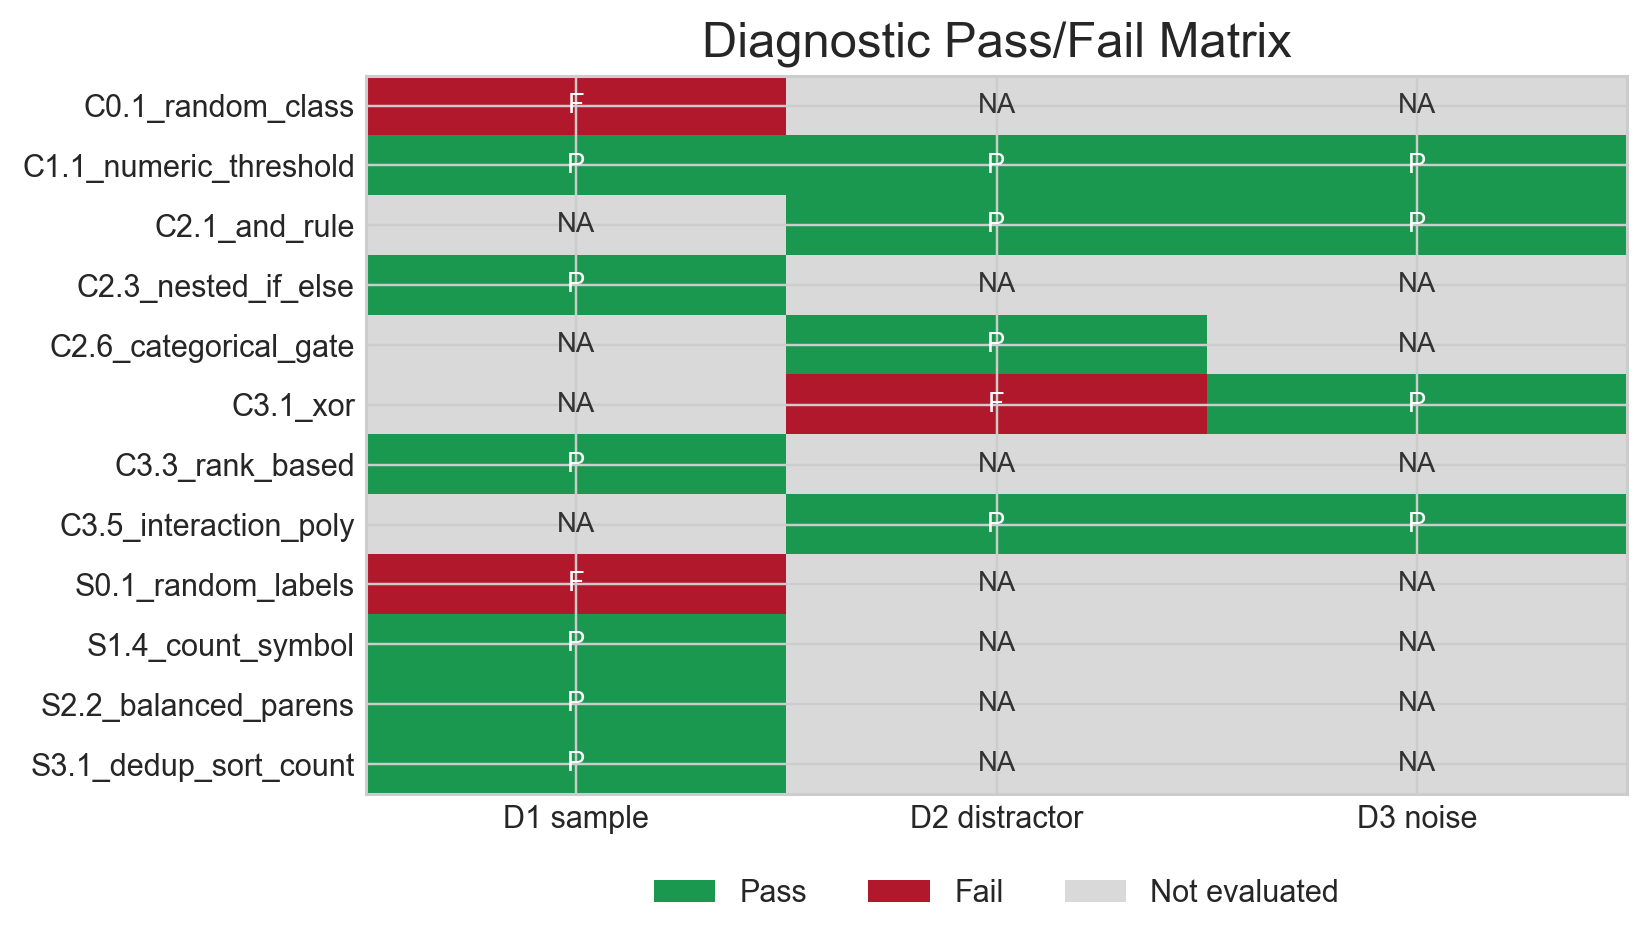
\includegraphics[width=0.88\textwidth]{diagnostic_matrix.png}
\caption{Diagnostic pass and fail matrix. Missing cells indicate ``not evaluated,'' not implicit success.}
\label{fig:diag}
\end{figure}

Diagnostics mostly reinforce the classification result section. Sample efficiency separates intended algorithmic tasks from controls, distractor robustness is strong on most tested classification tasks, noise robustness is uniformly strong on its tested subset, and feature-alignment results are clean on the currently evaluated task-model pairs. At the same time, the benchmark still exposes meaningful failures: \texttt{C3.1\_xor} fails distractor robustness, which is precisely the sort of brittleness that a benchmark of algorithmic solvability should surface.

The zero label changes in \texttt{EXP-D5} are not a disappointment. They are a consequence of the methodology repair that now routes the same D1/D2/D4 evidence into baseline reporting. Calibration is therefore confirmatory and consistency-checking rather than a second competing label path.

Table~\ref{tab:bonus} and Figure~\ref{fig:bonus} summarize the bonus symbolic-recovery stage.

\begin{table}[H]
\centering
\caption{Bonus symbolic recovery summary.}
\label{tab:bonus}
\begin{tabular}{lrrr}
\toprule
Experiment & Tasks evaluated & Tasks passing & Pass rate \\
\midrule
\texttt{EXP-B1} rule extraction & 12 & 9 & 0.7500 \\
\texttt{EXP-B2} program search & 9 & 7 & 0.7778 \\
\bottomrule
\end{tabular}
\end{table}

\begin{figure}[H]
\centering
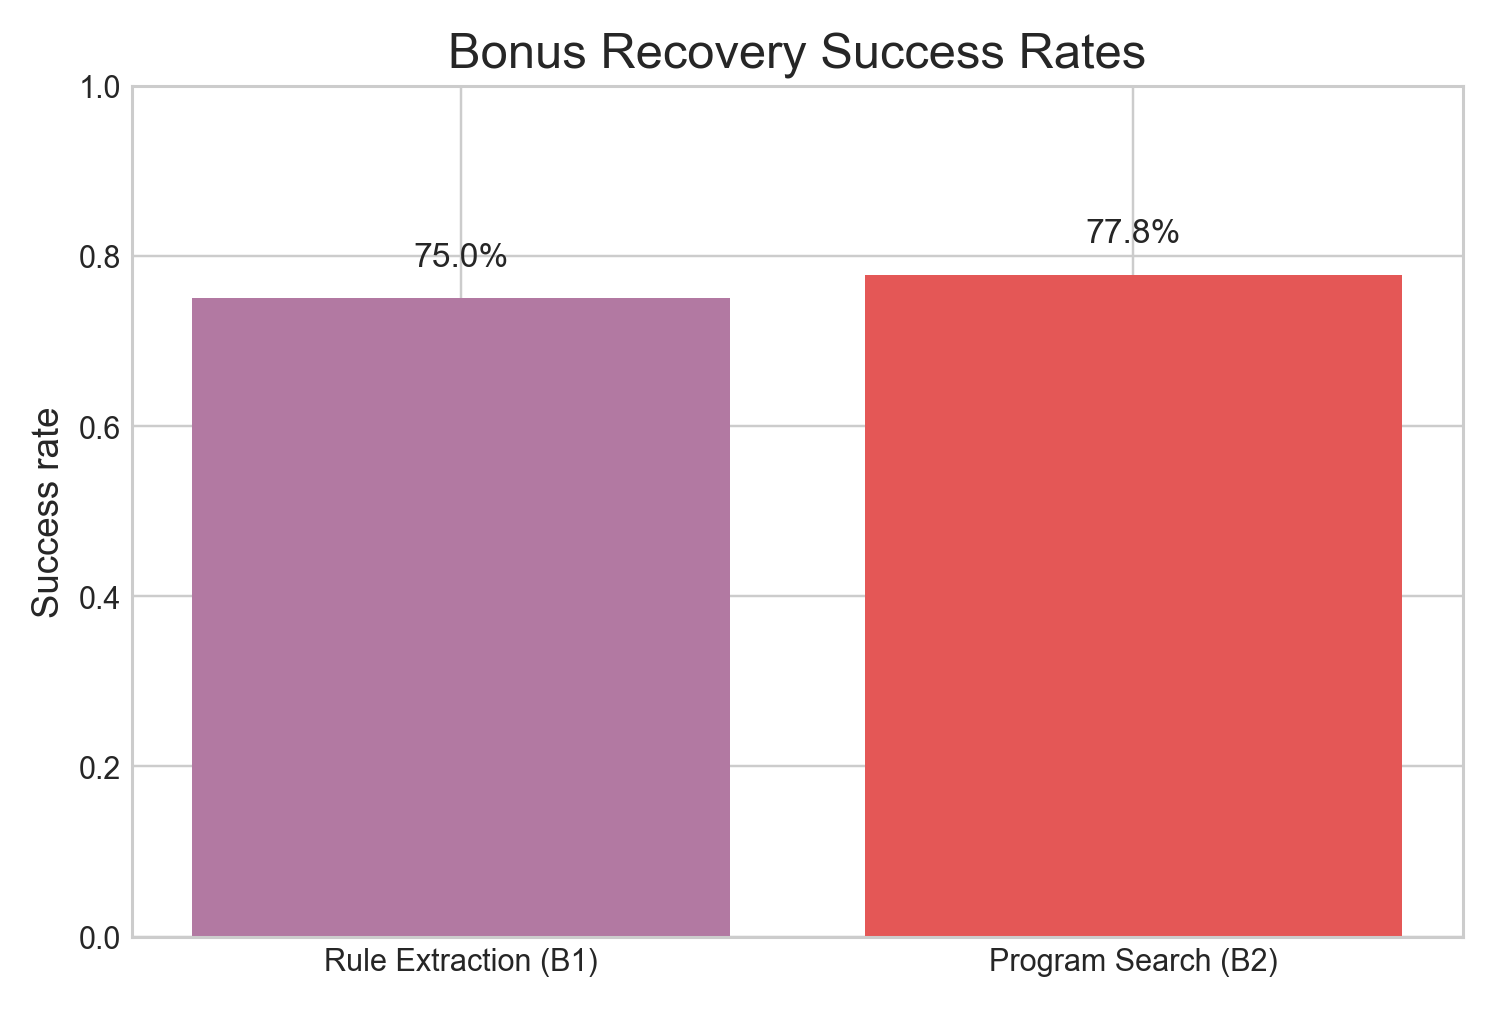
\includegraphics[width=0.66\textwidth]{bonus_success_rates.png}
\caption{Bonus symbolic recovery success rates. Symbolic recovery remains stronger than learned sequence generalization.}
\label{fig:bonus}
\end{figure}

This is a central interpretive result. If both learned models and symbolic search were failing, the benchmark tasks themselves would be suspect. Instead, symbolic recovery succeeds on most searched tasks. The more plausible reading is that the benchmark is algorithmically coherent, while the current learned sequence models remain weaker than the task family demands.

\section{Discussion and Limitations}

The paper now supports a precise and review-ready set of claims.

First, the classification track provides broad evidence of algorithmic solvability on the implemented deterministic tabular tasks. That claim is supported by the label distribution, by strong OOD behavior, and by diagnostics that mostly reinforce the baseline story.

Second, the sequence track is no longer well described by a blanket negative summary. Longer, regularized training clearly improves several tasks and reveals delayed held-out gains on others. However, the benchmark still does not support a broad positive claim about learned sequence algorithmic solvability under the executed model family.

Third, symbolic recovery remains stronger than learned sequence generalization. This matters because it shifts the burden of explanation away from benchmark incoherence and toward model-family limitations.

Several limitations should be disclosed directly.

\paragraph{Implemented scope.}
The evidence covers only \texttt{S0-S3} and \texttt{C0-C3}. Deferred tiers remain future work.

\paragraph{Model-family dependence.}
The weak sequence result is a statement about the currently executed model family, not about all possible sequence architectures. No Transformer, scratchpad, or trace-supervised sequence model is present in the current rerun.

\paragraph{Partial diagnostic coverage.}
Diagnostics evaluate targeted subsets rather than every task. Missing cells should be read as unevaluated, not as passing.

\paragraph{Training-stack warnings.}
The current stack is correctness-clean but not optimization-clean. Convergence warnings remain and should be treated as technical debt.

\paragraph{Baseline distractor evidence.}
Criterion 7 is still partly carried by diagnostics rather than by a native baseline distractor split, which remains an important follow-up for the classification track.

The next task is therefore straightforward: add native baseline distractor coverage, then move on to broader sequence-architecture expansion.

\section{Conclusion}

The current benchmark is already scientifically useful. It can distinguish strong from weak task families, expose nontrivial fragilities such as distractor sensitivity, and separate learned generalization from symbolic recoverability. After the latest methodology repairs, it also supports a more defensible paper narrative than the earlier prepublication draft.

The correct conclusion is neither that algorithmic solvability from examples is broadly solved nor that the benchmark has failed. Rather, the current evidence shows that deterministic tabular rule tasks are already tractable under standard models within the implemented scope, whereas learned symbolic sequence generalization remains the main unresolved regime. Longer training helps, but not enough. That makes the next stage of work clear: add baseline-native distractor coverage, then expand the sequence architecture and supervision stack without compromising the now-stable experimental and reporting pipeline.

\appendix

\section{Selected Task-Level Outcomes}

\begin{table}[H]
\centering
\caption{Selected task-level results that anchor the current paper's main claims.}
\label{tab:selected}
\begin{tabular}{llrrl}
\toprule
Task & Best model & Best IID & Best OOD & Label \\
\midrule
\texttt{C1.1\_numeric\_threshold} & decision tree & 1.000 & 1.000 & \texttt{STRONG} \\
\texttt{C2.6\_categorical\_gate} & decision tree & 0.999 & 1.000 & \texttt{STRONG} \\
\texttt{C2.1\_and\_rule} & random forest & 1.000 & 1.000 & \texttt{STRONG} \\
\texttt{C1.6\_modular\_class} & random forest & 0.829 & 0.773 & \texttt{INCONCLUSIVE} \\
\texttt{S1.4\_count\_symbol} & LSTM & 0.991 & 0.908 & \texttt{MODERATE} \\
\texttt{S1.5\_parity} & LSTM & 0.977 & 0.947 & \texttt{WEAK} \\
\texttt{S2.2\_balanced\_parens} & LSTM & 0.997 & 0.990 & \texttt{WEAK} \\
\texttt{S2.3\_running\_min} & LSTM & 0.644 & 0.000 & \texttt{INCONCLUSIVE} \\
\texttt{S1.2\_sort} & LSTM & 0.312 & 0.000 & \texttt{NEGATIVE} \\
\bottomrule
\end{tabular}
\end{table}

\begin{thebibliography}{9}

\bibitem{lake2018scan}
Brenden M. Lake and Marco Baroni.
\newblock Generalization without Systematicity: On the Compositional Skills of Sequence-to-Sequence Recurrent Networks.
\newblock In \emph{Proceedings of ICML}, 2018.

\bibitem{kim2020cogs}
Najoung Kim and Tal Linzen.
\newblock COGS: A Compositional Generalization Challenge Based on Semantic Interpretation.
\newblock In \emph{Proceedings of EMNLP}, 2020.

\bibitem{velickovic2021nar}
Petar Velickovic and Charles Blundell.
\newblock Neural Algorithmic Reasoning.
\newblock \emph{Patterns}, 2(7), 2021.

\bibitem{velickovic2022clrs}
Petar Velickovic, Adriana Romero, Pieter W. Battaglia, and others.
\newblock The CLRS Algorithmic Reasoning Benchmark.
\newblock In \emph{Proceedings of NeurIPS}, 2022.

\bibitem{power2022grokking}
Alethea Power, Yuri Burda, Harri Edwards, Igor Babuschkin, and Vedant Misra.
\newblock Grokking: Generalization Beyond Overfitting on Small Algorithmic Datasets.
\newblock \emph{arXiv preprint arXiv:2201.02177}, 2022.

\bibitem{grinsztajn2022tabular}
Léo Grinsztajn, Edouard Oyallon, and Gaël Varoquaux.
\newblock Why do tree-based models still outperform deep learning on tabular data?
\newblock \emph{arXiv preprint arXiv:2207.08815}, 2022.

\bibitem{balog2017deepcoder}
Matej Balog, Alexander L. Gaunt, Marc Brockschmidt, Sebastian Nowozin, and Daniel Tarlow.
\newblock DeepCoder: Learning to Write Programs.
\newblock In \emph{Proceedings of ICLR}, 2017.

\end{thebibliography}

\end{document}
